\chapter{Síntesis lógica de un microprocesador RISC-V}
\label{ch:asp_syn}

En este capítulo se explica el proceso seguido para la síntesis lógica del código \textit{RTL} del microprocesador \textit{RISC-V} de aplicación específica desarrollado por el M.Sc. Carlos Salazar \cite{Carlosthesis}. En esencia la tarea encomendada consistía en efectuar la síntesis lógica del microprocesador y comprobar mediante simulaciones post síntesis lógica su funcionabilidad.

El \textit{ASP} diseñado por el M.Sc Salazar, tiene como propósito ejecutar un algoritmo de modelos ocultos de Marcov (\textit{HMM}), para la detección de patrones acústicos de disparos y motosierras dentro de ambientes boscosos. Explicar este algoritmo está más allá del objetivo de este trabajo, por lo que se invita al lector a referirse al trabajo \cite{Carlosthesis} si se desea profundizar más en el tema. Exponer el funcionamiento del \textit{RTL} del \textit{ASP} también queda por fuera del alcance de este trabajo. En consecuencia a lo anterior cabe mencionar que se parte de un código considerado correcto y con base en él se procede con la integración según el flujo de diseño de circuitos digitales expuesto en el capítulo anterior. 

%\section{Escenario de implementación}

En la figura \ref{fig:micro}, observamos la estructura del microprocesador que debía ser síntetizado, el \textit{RTL} de este dispositivo mantiene una estructura equivalente a la de la figura \ref{fig:micro}; sin embargo, a primera impresión es posible encontrar una gran deficiencia en el diagrama de bloques mostrado. Esta deficiencia consiste en la ausencia de un hardware que permita cargarle información en las memorias. Al analizar el código del M.Sc. Salazar se encontró que las memorias utilizadas fueron definidas desde la persepectiva de ser usadas en una tarjeta de desarrollo \textit{FPGA}, este dispositivo permite cargar las memorias pues cuenta con hardware y software capacitado para dicho fin.

\begin{figure}[t]
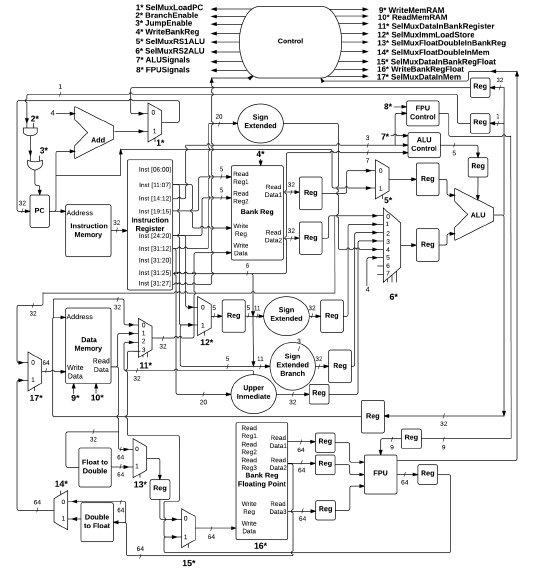
\includegraphics[width=\textwidth]{Micro.jpg}
\centering
\caption{Microprocesador ASP. RISC-V. Imágen replicada de \cite{Carlosthesis}, con la autorización del M.Sc Salazar.}
\label{fig:micro}
\end{figure}

La estructura del \textit{RTL} de las memorias consiste en desarrollar pequeños bloques de memorias de 8 bits y generar un bloque de memoria total de 32 bits. La técnica de codificación usada corresponde a un arreglo bidimensional en verilog. En el caso de la memoria de programa o instrucciones, se crea un bloque de memoria de 32 Kbytes (kilo bytes), y se replica 4 veces para tener una memoria de 32 Kbytes con un tamaño de palabra de 32 bits, de forma similar sucede con la memoria de datos.

Sintetizar esta estructura de memorias en la herramienta es no es viable debido al enorme volumen de registros que se debe utilizar, y sin una estructura definida para guiar a la herramienta de síntesis, se obtendrá como resultado un \textit{GLN} deficiente. Es por ello que conviene incluir bloques de memoria SRAM, que correponde a una estructura de memoria más eficiente.

Considerando la meta del proyecto, la cual es desarrollar un ASIC de bajo consumo, integrar memorias tan grandes implica mal lograr el espacio de silicio disponible para el chip. Por otra parte ausencia del harware para programar las memorias compromete la correcta implementación del proyecto, pues las mismas aunque puedan ser sintetizadas por la herramienta, no podrán ser inicializadas de forma correcta, en etapas posteriores.

Existe una particularidad extra a este proyecto, y consiste en que la unidad de punto flotante original fue desarrollada por el Ing. Diego Rodríguez \cite{Diego2015}; sin embargo, el diseño tenía muchas oportunidades de mejora, es por ello que fue optimizada por el Ing. Francis López \cite{Francis2016}. Esta última no fue probada junto al microprocesador, aunque se demostró su funcionabilidad de forma individual.

Resolver los problemas asociados al banco de memoria del microprocesador y cualquier discrepancia de conectividad y sincronicidad del \textit{RTL} está más allá del alcance de este trabajo. Recordando el objetivo general de este trabajo, el cual es la implementación de un flujo de diseño digital en las herramientas de \textit{Synopsys} y para demostrar su funcionalidad se usa el \textit{RTL} del microprocesador en cuestión, es decir se pretende implementar el microprocesador ASP en una tecnología CMOS de 0,13 micrómetros, no se pretende garantizar la funcionalidad del mismo, la optimización del RTL está fuera de la visión de este trabajo.

\section{Estrategia de síntesis y validación}

Recordando, el primer objetivo específico de este trabajo, que corresponde a efectuar la síntesis lógica de el \textit{RTL} del \textit{ASP}, y habiendo definido en el capítulo \ref{ch:scripting} el flujo de diseño digital, se tiene en consecuencia que debe someterse el código \textit{RTL} a las herramientas de \textit{FrontEnd}. El flujo ya fue expuesto en el capítulo anterior, así que no se entrará en detalles sobre como fue sometido el código, pero se hablará de las configuraciones y consideraciones que se establecieron para que la implementación tenga coherencia con lo esperado del diseño.

\subsection{Restricciones del diseño}
\label{s_sec:const}

Lo expuesto a continuación corresponde a los criterios usados en el scritp de \textit{TCL} de constraints (restricciones) expuesto en la sección \ref{script_syn}. Y este es uno de los puntos de partida fundamentales para la síntesis lógica del ASP.

\subsubsection{Modelo de carga en el cableado (wire\_load\_model)}
El modelo de cableado utilizado en este diseño corresponde al ibm13\_wl10 de la biblioteca scx3\_cmos8rf\_lpvt\_tt\_1p2v\_25c. La forma para determinar los modelos de cableado se hace mediante la herramienta \textit{Design Compiler} y solicitando el reporte de la biblioteca; sin embargo, se debe tener funcionando de forma correcta el \textit{Library Compiler}. Existen varias modalidades de configuración para el modelo de cableado, en los diseños trabajados en este proyecto se utiliza el modelo "top".

En el modo superior "top", el compilador de diseño modela las redes como si el diseño no tuviese jerarquía y utiliza el modelo de carga de cable especificado para el nivel superior de la jerarquía de diseño de todas las redes en un diseño y sus subdiseños. La herramienta ignora todos los modelos de carga de cable configurados en subdiseños con el comando set\_wire\_load\_model.

\subsubsection{Reloj y factor de actividad}

Los diseños se diseñan previendo una frecuencia de operación general de 100 MHz por lo que se crea un reloj de con un periodo de 10 ns. Con el fin de modelar un reloj más realista se especifica una transición de 0.5 ns, lo cual se traduce como una pendiente en los flancos de subida y bajada del reloj.

También se específica una incertidumbre (skew) con márgenes de setup y de hold de 0.5 ns, esto corresponde al lapso entre dos flancos sucesivos con respecto a la variación fuera de los tiempos de llegada nominales. Finalmente se especifica una latencia de 0.5 ns, y es básicamente un parámetro que le indica a la herramienta el lapso que se da desde que la señal conmuta en su fuente hasta que conmuta en la entrada de una celda, y su utilidad es sólo para fines de análisis de sincronía y simulación dinámica.

Asociado indirectamente al reloj se encuentra el factor de actividad que le sirve a las herramientas, efectuar el análisis de potencia. Este parámetro se configura con una razón de conmutación del 25\% y una probabilidad estática del 50\% pues el reloj es simétrico.

\subsubsection{Puertos y propagación de señales}

Las señales de reloj y reset se configuran para que en ellas se coloquen la mínima cantidad de búfers, y que en general las señales se intervengan de forma mínima en la síntesis. 

Se configura un intervalo de retraso en la propagación de los puertos, con el fin de que los análisis y la simulación sean más realistas, en el caso de las entradas el retardo es 1 ns como mínimo y de 3.5 ns como máximo, y de 1 a 2 ns para las salidas.

Los modelos de la carga asociada a las salidas y entradas se establecen en función de la celda de conducción (driving\_cell), esta configuración le permite a la herramienta de análisis de sincronía estimar de forma precisa el retraso causado desde la conmutación en un puerto, y sobre toda la ruta de propagación consecuente.

Se usa 10 la máxima cantidad de fanout permitda para los puertos de entrada, esto con el fin de que durante la síntesis la herramienta garantice que la cantidad de cargas conectadas directamente a esos puertos, no sobrepase un valor determinado.

\subsection{Comprobación de la síntesis}
\label{sec:comp_syn}
Como ya se mencionó el diseño del M.Sc Salazar, presenta algunas deficiencias a la hora de considerar someterlo al flujo de diseño digital. En respuesta a lo anterior se efectuó el siguiente proceso.

\begin{enumerate}

\item En primer lugar se modificó el RTL haciendo un bypass\footnote{Bypass: anglicismo para aludir a un cambio de ruta o desvío en una ruta} en la conexión de la memorias, creando puertos para conectar de forma externa las memorias con los módulos que las instanciaban originalmente.

\item Se tomó el RTL original con la FPU diseñado por el Ing. Rodríguez, y se estimuló de acuerdo con el banco de pruebas (testbench) proporcionado junto al RTL del ASP. Esta simulación por comportamiento se define como la referencia dorada para validar el diseño.

\item Luego se sustituye la FPU por la diseñada por el Ing. López y se estimula el ASP de nuevo en una simulación por comportamiento para valorar la congruencia con el diseño original.

\item Se sintetiza entonces el RTL sin el banco de memorias, ya que como se mencionó anteriormente, incluir las memorias tal cual se diseñaron en la síntesis, es considerablemente engorroso e ineficiente.

\item Se realiza una simulación post síntesis lógica del ASP usando un estrategia de simulación hibrida, en el sentido de que se convinarán elementos de RTL (modelos por comportamiento) y elementos GLN (modelos post síntesis). Así se pretende modelar las memorias como elementos ideales y poder comprobar la funcionalidad del ASP.
\end{enumerate}

\section{Resultados de la síntesis lógica del ASP.}

Habiendo definido el entorno particular en el que se recibió el RTL y las consideraciones que se tomaron para poder comprobar la correcta síntesis del mismo, se muestran los siguientes resultados ofrecidos por los reportes de la herramienta.

\newpage

\subsection{Reportes generados en el proceso de síntesis lógica}
\begin{table}[ht]
\centering
\label{tab:power_asp}
\caption{Resumen del reporte de potencia del microprocesador ASP post síntesis lógica}
\begin{tabular}{||l | c | c | c | c | c |}
\hline
\hline
Group & Internal & Switching  & Leakage & Total & \% Attrs \\
\hline
io\_pad & 0.0000 & 0.0000 & 0.0000 & 0.0000 & 0.00\% \\
\hline
memory & 0.0000 & 0.0000 & 0.0000 & 0.0000 & 0.00\% \\
\hline
black\_box & 0.0000 & 0.0000 & 0.0000 & 0.0000 & 0.00\% \\
\hline
clock\_network & 0.0000 & 0.0000 & 0.0000 & 0.0000 & 0.00\% \\
\hline
register & 7.9920 & 4.2648e-02 & 1.7974e+05 & 8.0349 & 84.01\%\\
\hline
sequential  & 0.0000 & 0.0000 & 0.0000 & 0.0000 & 0.00\% \\
\hline
combinational & 0.1635 & 1.3654 & 3.6572e+05 & 1.5293 & 15.99\% \\
\hline
Total &  8.1556 mW & 1.4081 mW & 545.4596 nW & 9.5642 mW & 100 \%\\
\hline
\hline
\end{tabular}
\end{table}

%\newpage
\begin{lstlisting}[caption={Reporte de área del microprocesador ASP post síntesis lógica.} \label{lst:asp_area_report}, frame={single}]
****************************************
Report : area
Design : MainHMM_2
Version: L-2016.03-SP3
Date   : Wed Dec 14 13:21:38 2016
****************************************

	Library(s) Used: scx3_cmos8rf_lpvt_tt_1p2v_25c

          Number of ports:                          920
          Number of nets:                         40225
          Number of cells:                        37979
          Number of combinational cells:          32684
          Number of sequential cells:              5293
          Number of macros/black boxes:               0
          Number of buf/inv:                       8740
          Number of references:                      40

          Combinational area:             318738.243849
          Buf/Inv area:                    49842.720788
          Noncombinational area:          139687.197126
          Macro/Black Box area:                0.000000
          Net Interconnect area:         4646623.786163

          Total cell area:                458425.440975
          Total area:                    5105049.227139
\end{lstlisting}

\newpage

\begin{lstlisting}[caption={Reporte de sincronía del microprocesador ASP post síntesis lógica.} \label{lst:asp_timing_report}, frame={single},basicstyle=\small]
****************************************
Report : timing -path full -delay max -max_paths 1
Design : MainHMM_2 Version: L-2016.03-SP3
****************************************
		Path Group: clk | Path Type: max
  ---------------------------------------------------------------
  Des/Clust/Port     Wire Load Model       Library
  MainHMM_2          ibm13_wl10     scx3_cmos8rf_lpvt_tt_1p2v_25c
  ---------------------------------------------------------------
  Point					Incr		Path
  clock clk (rise edge)			0.00		0.00
  clock network delay (ideal)		1.00		1.00
  $A/State_reg[3]/CK (DFFQX1TS)		0.00 #		1.00 r
  $A/State_reg[3]/Q (DFFQX1TS)		1.05		2.05 f
  CPUMain/U367/Y (INVX4TS)		0.53		2.59 r
  CPUMain/U2567/Y (INVX4TS)		0.49		3.08 f
  CPUMain/U235/Y (OR3X2TS)		0.68		3.76 f
  CPUMain/U972/Y (CLKINVX3TS)		0.57		4.32 r
  CPUMain/U180/Y (NOR2X1TS)		0.47		4.79 f
  CPUMain/U16337/Y (OAI222X4TS)		0.86		5.65 r
  CPUMain/U147/Y (NOR3BX1TS)		0.49		6.14 r
  CPUMain/U134/Y (BUFX3TS)		0.76		6.90 r
  CPUMain/U5970/Y (NOR2X4TS)		0.51		7.41 f
  CPUMain/U20520/Y (NOR2X2TS)		0.72		8.13 r
  CPUMain/U9888/Y (BUFX3TS)		0.88		9.01 r
  CPUMain/U6270/Y (BUFX3TS)		0.83		9.83 r
  CPUMain/U20522/Y (OAI22X1TS)		0.48		10.31 f
  $B/DataOutput_reg[0]/D (DFFQX1TS)	0.00		10.31 f
  data arrival time					10.31
  clock clk (rise edge)			10.00		10.00
  clock network delay (ideal) 		1.00		11.00
  clock uncertainty           		-0.50		10.50
  $B/DataOutput_reg[0]/CK (DFFQX1TS)	0.00		10.50 r
  library setup time			-0.19		10.31
  data required time					0.31
  ---------------------------------------------------------------
  data required time					10.31
  data arrival time					-10.31
  ---------------------------------------------------------------
  slack (MET)						0.00
  ---------------------------------------------------------------
  Notes:
  	$A = CPUMain/ExtensionFloat.FSMControlCPUFloatPoint
  	$B = CPUMain/BankRegisterInteger/Registro5_t0
\end{lstlisting}

\newpage

\subsection{Simulaciones}
\subsubsection{Referencia Dorada}

\begin{figure}[ht]
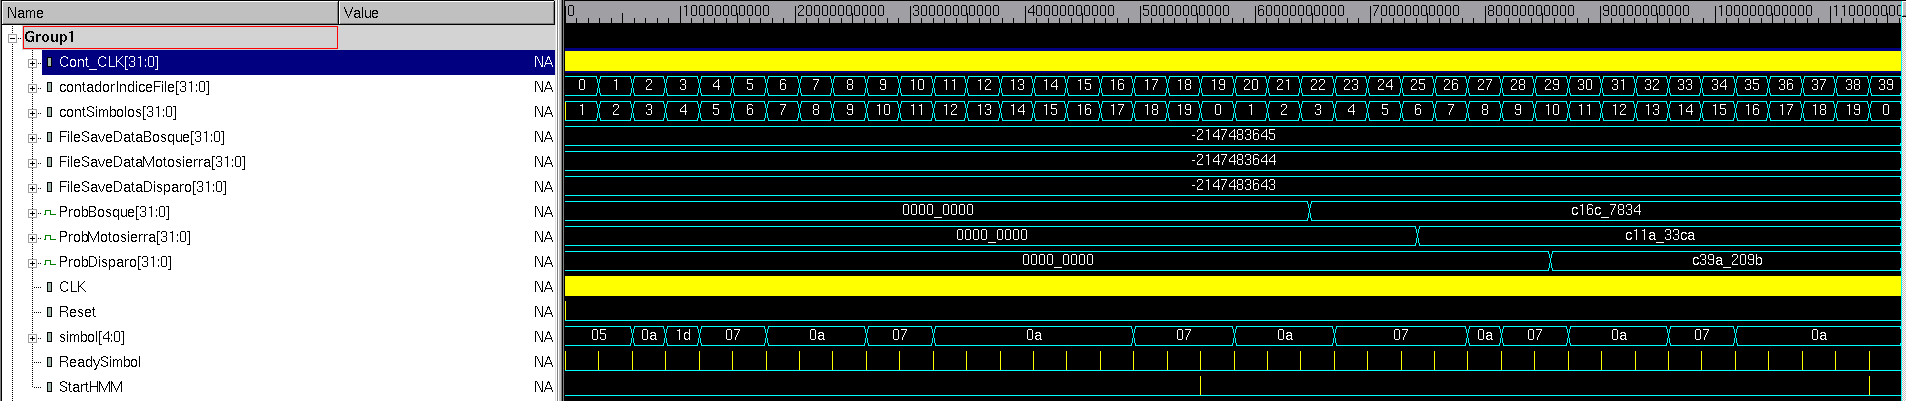
\includegraphics[width=\textwidth]{GR_sim.png}
\centering
\caption{Resultado de la simulación por comportamiento del ASP con la FPU diseñada por el Ing. Rodríguez. Según lo estipulado por el M.Sc Salazare en \cite{Carlosthesis}, este, es el comportamiento esperable del ASP, al ejecutar el algoritmo HMM.}
\label{fig:gr_sim}
\end{figure}

\subsubsection{Algoritmo HMM ejecutado en el ASP}
\begin{figure}[ht]
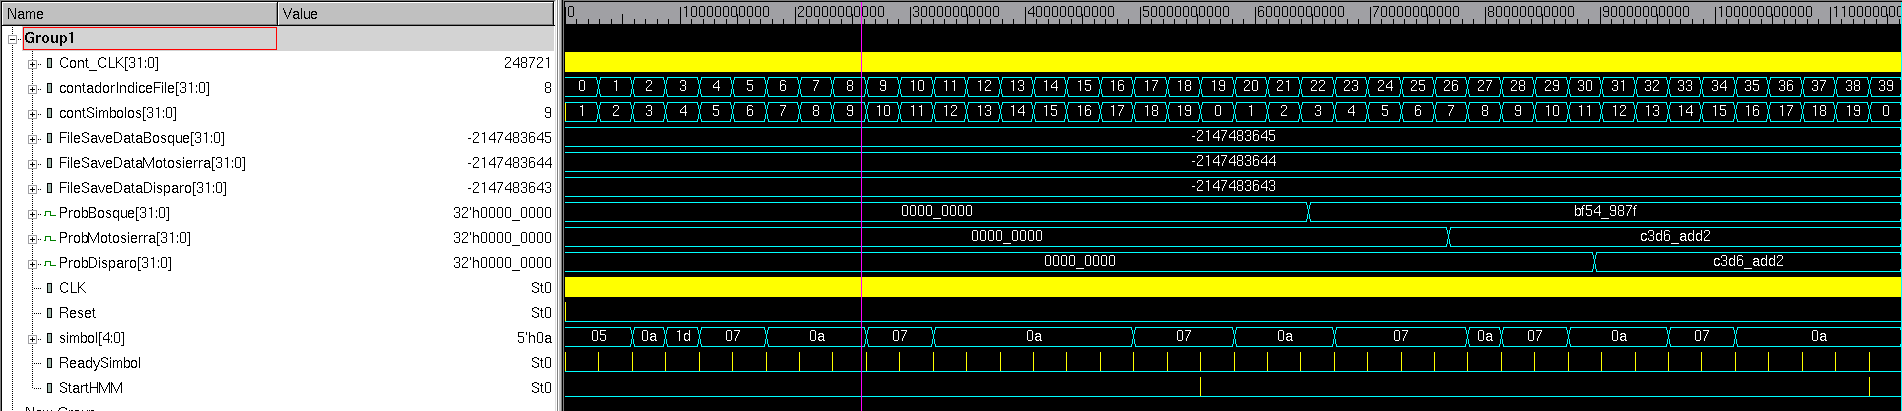
\includegraphics[width=\textwidth]{asp_beh_sim.png}
\centering
\caption{Resultado de la simulación por comportamiento del ASP con la FPU diseñada por el Ing. López.}
\label{fig:asp_beh_sim}
\end{figure}

\begin{figure}[ht]
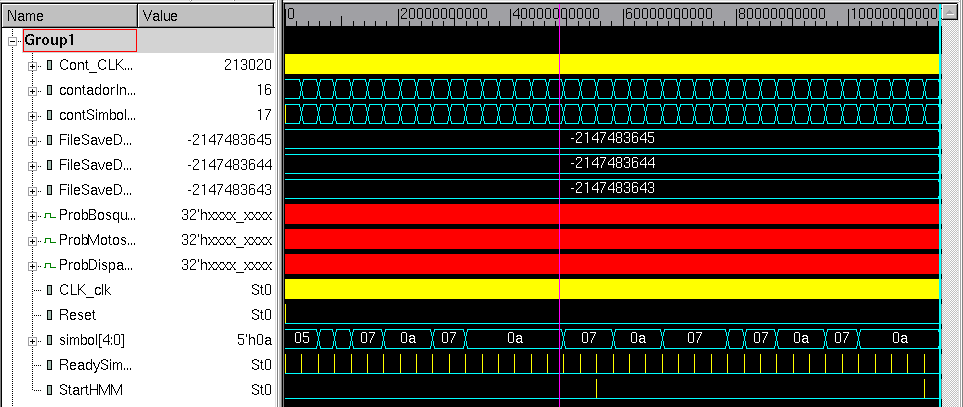
\includegraphics[width=\textwidth]{asp_syn_sim.png}
\centering
\caption{Resultado de la simulación post síntesis lógica del ASP con la FPU diseñada por el Ing. López.}
\label{fig:asp_syn_sim}
\end{figure}

\begin{figure}[ht]
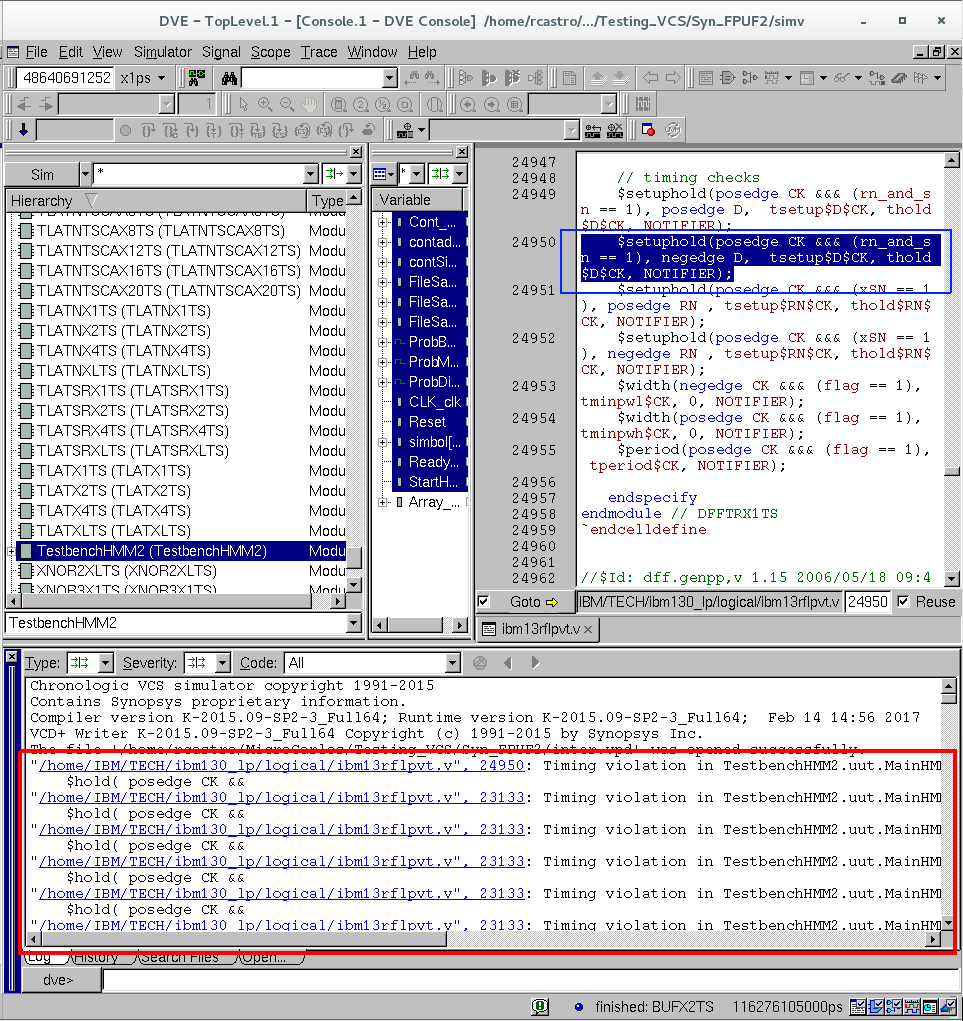
\includegraphics[width=\textwidth]{asp_hold_rape.png}
\caption{Foto captura de la información de la herramienta VCS al generar la simulación post síntesis del microprocesador ASP}
\label{fig_asp_hold}
\end{figure}

\section{Análisis de resultados: Síntesis Lógica del ASP}

\subsection{Evaluación pre síntesis}

Comenzando por el análisis a nivel de comportamiento del \textit{RTL} de los diseños, y considerando el diseño del \textit{ASP} que incorpora la \textit{FPU} del Ing. Rodríguez se presenta el siguiente escenario.

Los datos observados en las figuras \ref{fig:gr_sim}, \ref{fig:asp_beh_sim} \ref{fig:asp_syn_sim} correspondientes a los vectores de salida: ProbBosque, ProbMotosierra, y ProbDisparo son datos en hexadecimal, que representan un número en punto flotante de precisión simple, según el estándar IEEE574. Por lo tanto tenemos que para la figura \ref{fig:gr_sim}, según el estímulo usado (Definido en el testbench, aportado junto al \textit{RTL}) los valores corresponden a -14.779346 para ProbBosque, -9.637644 para ProbMotosierra , y -308.25473 para ProbDisparo.

Según expone el M.Sc Salazar en \cite{Carlosthesis} los valores puntualmente no corresponden a una estadística, pues no existen probabilidades negativas, por lo que estos valores son más una heurística que permite determinar que tan cercano se encuentra un dato a pertenecer a uno de los 3 conjuntos mencionados, y el criterio que los determina, consiste en qué tan cercanos se encuentren estos valores a cero. Observando que para la figura \ref{fig:gr_sim}, se aprecia que el valor más cercano a cero corresponde al vector ProbMotosierra, por lo tanto, el estímulo tiene una probabilidad más alta de pertenecer a un patrón acústico tipo motosierra; sin embargo, existe una probabilidad modesta de asociar el estímulo al patrón acústico del bosque, lo cual es esperable de acuerdo con las condiciones en las que fueron adquiridos los sonidos que se usaron como estímulos, finalmente observamos que el estímulo definitivamente no puede considerarse como un disparo, pues su valor se encuentra 2 ordenes de magnitud lejos del cero.

Lo anterior fue expuesto para ubicar al lector sobre la semántica de los datos, no se explicará a fondo pues discutir esos tópicos se encuentran por fuera del objetivo de este trabajo, si el lector lo desea puede referirse al trabajo \cite{Carlosthesis} para un comprensión más basta de la interpretación de estos datos.

Partiendo de la premisa de que el testbench contiene un estímulo que corresponde al patrón acústico de una motosierra, pués así fué especificado por el M.Sc Salazar al entregar el código \textit{RTL} y expuesto el tema del significado de los datos, se procede a efectuar un contraste entre las figuras \ref{fig:gr_sim}, \ref{fig:asp_beh_sim}. En este se puede encontrar que ProbBosque tiene un valor -0.8304519 (0xbf54987f), mientras que ProbMotosierra y ProbDisparo tienen un valor de -429.35797 (0xc3d6add2). Lo cual según el criterio expuesto anteriormente conduce a considerar que el estímulo es definitivamente sonido de bosque, pues los otros valores están muy lejos del cero. Conociendo que el estímulo en principio es un sonido asociado a una motosierra, y que la respuesta observada en la figura \ref{fig:gr_sim} es correcta, se establece que el \textit{ASP} que incorpora la \textit{FPU} del Ing. López funciona erróneamente. 

\subsection{Evaluación post síntesis}

No obstante a la discrepancia encontrada con las versiones del \textit{ASP}, y considerando que el objetivo de este trabajo es diseñar un flujo de diseño de circuitos integrados digitales, se somete el diseño al flujo en cuestión para poder evaluar los resultados del flujo y no el desempeño del \textit{ASP}.
%\ref{tab:power_asp}
Como puede observarse en la tabla 4.1 la red de reloj no consume energía, así tampoco los bloques de lógica secuencial, esto se debe a que al experimentar con el \textit{RTL} del microprocesador se encontraron las deficiencias en el \textit{RTL} comentadas anteriormente, por lo que se efectuó la compilación del diseño considerando una red de reloj ideal. Sin embargo el reporte de potencia permite identificar el grado de consumo de los distintos bloques en el diseño, y dado a que se extrajeron los bloques de memoria de este diseño, además de obligar a la herramienta a considerar la red de reloj como una red ideal observamos que el grueso del consumo lo tienen las categorías de registros y lógica combinacional.

El reporte de timing (sincronía), apreciado en el bloque de código \ref{lst:asp_timing_report}, permite observar el comportamiento de la red con el camino crítico, que como ya se mencionó es determinada dinámicamente por la herramienta durante el proceso de compilación en el flujo de la síntesis lógica. Nuevamente el reporte de timing permite apreciar que la red de reloj tiene un comportamiento ideal. Presenta una tabla donde en la primer columna indica la celda por la que atraviesa la señal (dato) del camino, la segunda columna indica cuanto retraso aporta a la red, y el tercero indica cuanto retardo se ha acumulado, hasta definir el tiempo que una señal (dato) tarda en propagarse a través del camino crítico (data arrival time).

Finalmente en el reporte de timing se consideran los atributos de la red de reloj que se definieron en las restricciones de síntesis, y se define un tiempo límite en el que el dato debería llegar (data required time), la diferencia entre el tiempo requerido y el tiempo de arrivo del dato establecen el \textit{Slack}, este parámetro indica si un diseño es capaz de funcionar correctamente a la velocidad requerida, es deseable tener un slack mayor o igual a cero. Como se puede observar este diseño cumple justamente el slack, lo cual es aceptable, aunque suelen ser deseables slacks positivos.

Como puede observarse en la simulación post síntesis, las señales correspondientes a los vectores a:
ProbBosque, ProbMotosierra, y ProbDisparo, se encuentran en estado indeterminado ("x"), evidentemente esto quiere decir que el modelo \textit{GLN} generado en la síntesis lógica no está funcionando de la misma manera en que lo hace el \textit{RTL}; sin embargo, no quiere decir que el producto de la síntesis sea erróneo.

Considerando el escenario de establecido al principio de este capítulo donde se definió que para poder efectuar la síntesis lógica, se iban a extraer los bloques de memoria del microprocesador, y como se planteó posteriormente en la sección \ref{sec:comp_syn} que el proceso de síntesis iba a culminar con una simulación mixta, en el sentido de que se iba a usar el \textit{RTL} original de los bloques de memorias, junto al \textit{GLN} generado por la herramienta de síntesis, es de esperar que el diseño no funcione adecuadamente. Pues una simulación post síntesis trata precisamente de incluir efectos de retardo de las señales que el \textit{RTL} no ofrece.

En la figura \ref{fig_asp_hold} se observa una captura de los mensajes que ofrece la herramienta al compilar la simulación deseada, como puede apreciarse en la ventana de mensajes, que ha sido resaltada con un recuadro rojo, para este diseño se observa una enorme cantidad de errores de "hold", y  en escencia quiere decir que el tiempo de hold para un no se cumple para un registro dado, que es indicado por la herramienta en la ventana de dependencias, en la imagen se resalta uno de los registros en cuestión mediante un recuadro azul.

Este tipo de errores pueden tener distintas fuentes; sin embargo, el reporte de timing indica que el slack se cumple para el camino crítico, podría analizarse si alguno de estos registros pertenece al camino crítico y a lo mejor realizar una optimización en el proceso de síntesis. También es posible usar la herramienta para STA y generar un panoráma más amplio sobre que sucede puntualmente con el diseño. Pero partiendo del hecho de que se está realizando una simulación enfocada a un código en \textit{GLN}, en la que se ha mezclado \textit{RTL} sin información de retardos y que el diseño se probó erróneo mediante las simulaciones por comportamiento, no es viable intentar optimizarlo.

Recapitulando lo expuesto en los 4 párrafos anteriores, la simulación observada en la figura \ref{fig:asp_syn_sim} indica que el diseño no se comporta según lo esperado y la figura \ref{fig_asp_hold} establece que existen múltiples fuentes de error, asociadas a problemas de hold, que considerando el escenario de síntesis son esperables de acuerdo con las condiciones en las que fue efectuada la síntesis y se genera la simulación.

Finalmente en el bloque de codigo \ref{lst:asp_area_report} se observa el reporte de área, que es un compendio de la cantidad de elementos y su categoría dentro de la biblioteca, abstrayendo su información en términos de espacio, por lo que permite generar un modelo estimado del área necesaria para generar el layout del diseño. Esta información se muestra con mayor relevancia en el capítulo siguiente.


